\documentclass[a4paper]{article}
\usepackage{graphics}
\usepackage{epsfig}
%\usepackage{graphicx}
\usepackage{sverb}
\usepackage{verbatim}
\usepackage{url}
\usepackage{float}
\usepackage{fancyhdr}
\usepackage{wrapfig}
\usepackage[utf8]{inputenc}
\providecommand{\OO}[1]{\operatorname{O}\left(#1\right)}

\pagestyle{fancy}
\fancyhead{}
\fancyfoot{}
\fancyfoot[CO,CE]{Author: Robert Foss - 8707174051 \\ \thepage}
\renewcommand{\headrulewidth}{0pt}
\title{Project 2\\ FMN011}
\author{Robert Foss (dt08rf1@student.lth.se)}
\date{} % Blir dagens datum om det utel�mnas

\begin{document} % B�rjan p� dokumentet
\maketitle
\thispagestyle{empty}
\newpage
\tableofcontents
\thispagestyle{empty}
\newpage

% \begin{EPIC TEXT}



\section{Introduction and problem background}
The issue of drawing  B�zier curves involves iterative calculation of points that lie on a curve. Due to the iteration a computational approach is the easiest way to visually represent a B�zier curve.

\begin{comment}Briefly  describe the general problem you want to solve and why a numerical or computational solution (as opposed to an exclusively analytical  solution) is required.
\end{comment}



\section{Numerical Considerations}
Points in B�zier curves were with found with de Casteljau's algorithm. The algorithm was implemented in Matlab and can be found in appendix A, section \ref{casteljau}. Specific Matlab functions used include flipud, rectint, cell matrices, saveas, axis and set.
\begin{comment}
Briefly  discuss the specific methods, software or algorithms you selected for  this problem. Mention any specific features of MATLAB you exploited.
\end{comment}

\section{Results}
\subsection{Task 1}
\subsubsection{Computational cost as per definition}
\begin{tabular}{lcccr}
$P(t) = \sum_{k=0}^{m}P_{k}B_{k}^{m}(t)$ & & & & $ B_{k}^{m} = \frac{m!}{k!(m-k)!}t^{k}(1-t)^{m-k} $
\end{tabular}
\\
\\
The number of operations for each factorial is $n-1$ given $n!$. The same applies to exponential expression such as $n^k$ which requires $k-1$ operations.
The calculation of a Bernstein polynomial of degree m requires 3m+2 operations.

The summation requires $m+1$ calculations of $P_{k}B_{k}^{m}(t)$. $P_{k}B_{k}^{m}(t)$ requires 2 calculations, one for each coordinate of the point. The actual summation requiers $m$ operations \rightarrow $(m+1) \cdot (3m+3) + m = 3m^{2} + 7m + 3$. That is \OO{m^2}.

\subsubsection{Computational cost of de Casteljau's algorithm}
de Casteljau's algorithm:
\\
\begin{tabular}{llllll}
\multicolumn{3}{l}{for j=1:m}&&&\\
&\multicolumn{3}{l}{for i=0:m-j}&&\\
&&\multicolumn{3}{l}{$P_{i}^{j} = P_{i}^{j-1}+(P_{i+1}^{j-1}-P_{i}^{j-1})t_{0}$}&\\
\end{tabular}
\\
\\
The work carried out in the inner loop is $(m-1)+(m-2)+..+1$, which can be represented with the geometric sum $\frac{(m-1)m}{2}$. 3 operations are carried for each point totaling 3*2 operations. Totaling $3\frac{(m-1)m}{2} = 3m^2 - 3m$ number fo operations.

\subsection{Task 2}
The implementation of de Casteljau's algorithm can be found in appendix A, section \ref{casteljau}. A secondary help function used for calculating multiple points of a B�zier curve was implemented and can be found in appendix A, section \ref{wrap}. Resulting plots can be found in appendix B, section \ref{task2}. Program listing can be found in appendix C, section \ref{programlisting}.

\subsection{Task 3}
Resulting plots can be found in appendix B, section \ref{task3a}, \ref{task3b}, \ref{task3c}, \ref{task3d} and \ref{task3e}. Program listing can be found in appendix C, section \ref{programlisting}. Points used were chosen experimentally and verified visually in the plots.

\subsection{Task 4}
Resulting plots can be found in appendix B, section \ref{task4a} and \ref{task4b}. Program listing can be found in appendix C, section \ref{programlisting}. The first set of control points used in a) ended where the second set of control points began. Resulting in a sharp angle. In b) the end of the first set of control points were made to have the same differential quotient as the beginning of the second set of control points. Resulting in a smooth link.

\subsection{Task 5}
Resulting plots can be found in appendix B, section \ref{task5}. Program listing can be found in appendix C, section \ref{programlisting}.

\subsection{Task 6}
The implementation of the splitting functions can be found in appendix A, section \ref{splitlower} and \ref{splitupper}. Resulting plots can be found in appendix B, section \ref{task6}. Program listing can be found in appendix C, section \ref{programlisting}.

\subsection{Task 7}
The implementation of the rectangle function can be found in appendix A, section \ref{box}. Resulting plots can be found in appendix B, section \ref{task7}. Program listing can be found in appendix C, section \ref{programlisting}.

\subsection{Task 8}
An implementation of the intersection detecting function can be found in appendix A, section \ref{intersection}. Resulting plots can be found in appendix B, section \ref{task8}. Program listing can be found in appendix C, section \ref{programlisting}.

\subsection{Task 9}
Resulting plots can be found in appendix B, section \ref{task9a} and \ref{task9b}. Program listing can be found in appendix C, section \ref{programlisting}.

\subsection{Task 10}
Resulting plots can be found in appendix B, section \ref{task10a} and \ref{task10b}. Program listing can be found in appendix C, section \ref{programlisting}. A lower case 'f' was chosen due to the longhand capital 'f' using multiple lines.

\section{Analysis}
Understanding the way the splitting function works was difficult was somewhat time-consuming.

The performance of the intersection method is not optimal as every splitted set of control points of the first curve were compared against every splitted set of control points of the second curve. The resulting performance is bad as large number of comparisons need to be made. However the performance was somewhat improved by jumping to the next iteration of the function as soon as a collision was detected


\begin{comment}
Include  a solid discussion and analysis of the results presented.  The  discussion should address any difficulties you encountered, appropriate  measures of performance (such as errors and computer time) and the  apparent sources of error you observed.
\end{comment}


\section{Lessons learned}
A few new Matlab functions were learned as noted in the numerical considerations section. The most useful being cell-matrices, that were used as an array of matrices.

Hands on experience with building curves to a certain specification.

I learned an iterative method of calculating intersections using rectangles and splitting.
\begin{comment}
Elaborate  a critical evaluation of the software you used. Make a list of the  specific things you  learned by working out the assignment, both  theoretical and practical issues.
\end{comment}

\section{Acknowledgements}
Angelica Gabasio, Mikael Nilsson and Mikael Sahlstr�m. \\
\emph{Numerical Analysis}, Timothy Sauer. Pearson Education, 2005.  

 \begin{comment}
 Mention  discussions  with other students or  teachers, software downloaded from  the web  or  copied from a book, and  any other relevant information you  find  fit to disclose.
 \end{comment}


\newpage

\section{Appendix: A}
\subsection{de Casteljau}
\label{casteljau}
\scriptsize
\verbatiminput{decasteljau.m}
\normalsize

\subsection{Wrap}
\label{wrap}
\scriptsize
\verbatiminput{wrap.m}
\normalsize

\subsection{Split lower}
\label{splitlower}
\scriptsize
\verbatiminput{splitlower.m}
\normalsize

\subsection{Split upper}
\label{splitupper}
\scriptsize
\verbatiminput{splitupper.m}
\normalsize

\subsection{Box}
\label{box}
\scriptsize
\verbatiminput{box.m}
\normalsize

\subsection{Intersection}
\label{intersection}
\scriptsize
\verbatiminput{intersection.m}
\normalsize

\newpage

\section{Appendix: B}
\subsection{Task 2}
\label{task2}
\begin{figure}[H]
\begin{center}
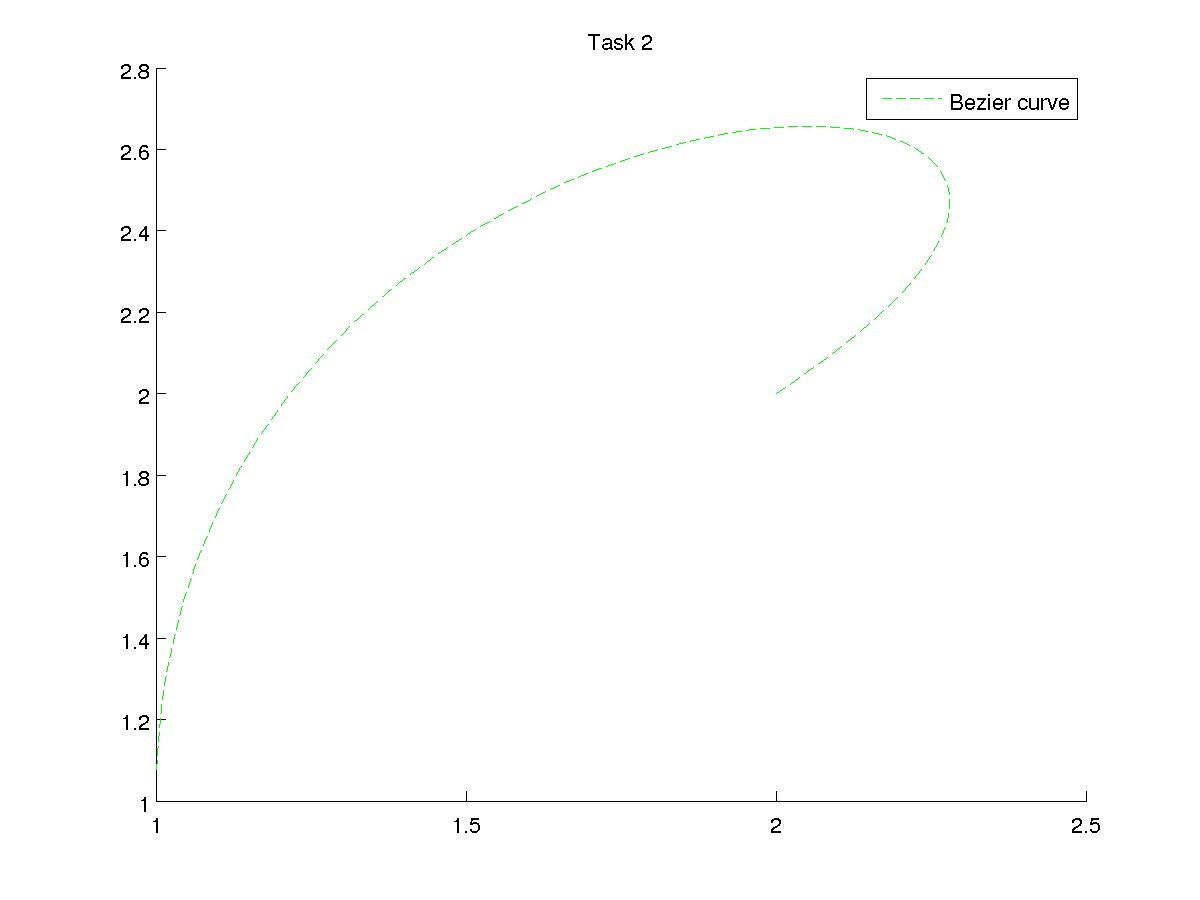
\includegraphics[scale=0.5]{task2.jpg}
\end{center}
\end{figure}

\subsection{Task 3a}
 \label{task3a}
 \begin{figure}[H]
 \begin{center}
 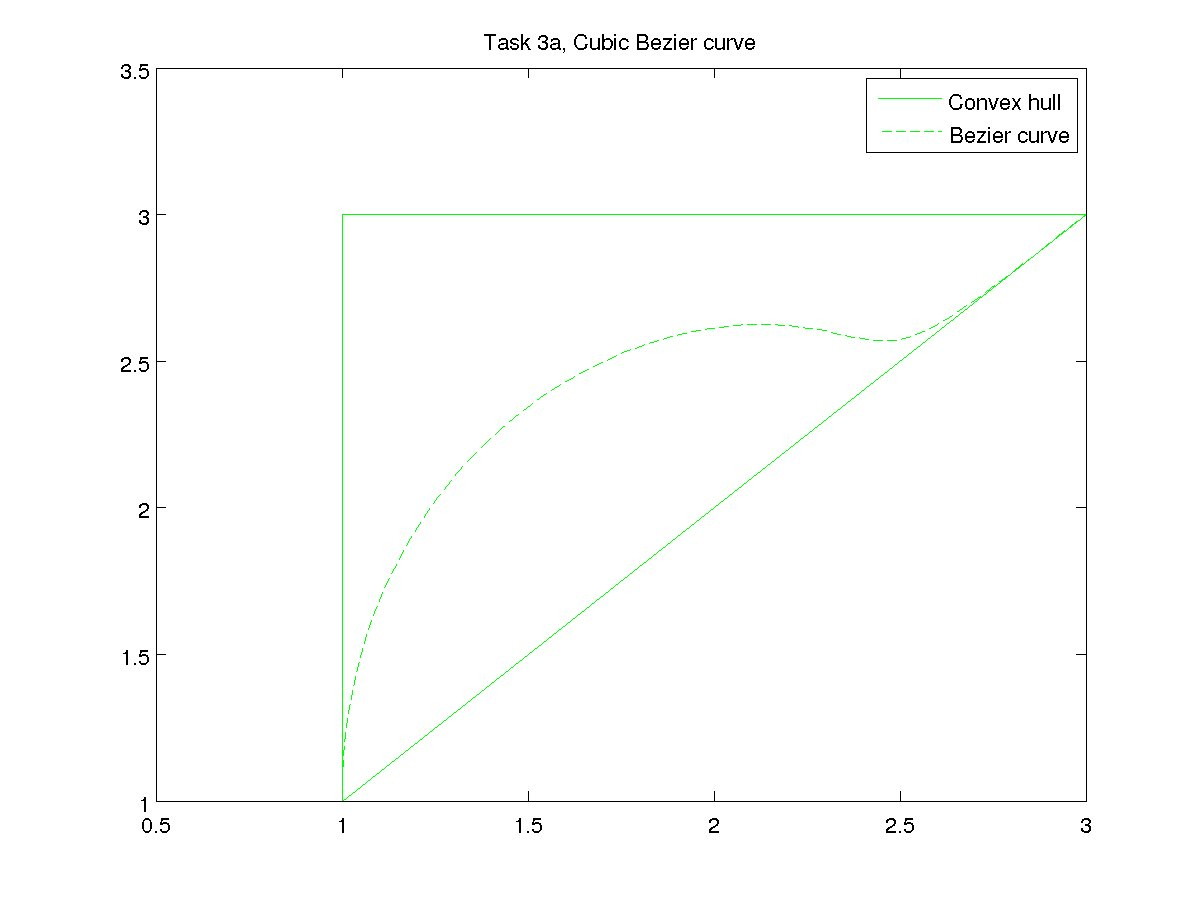
\includegraphics[scale=0.5]{task3a.jpg}
 \end{center}
 \end{figure}
\newpage

 \subsection{Task 3b}
\label{task3b}
\begin{figure}[H]
\begin{center}
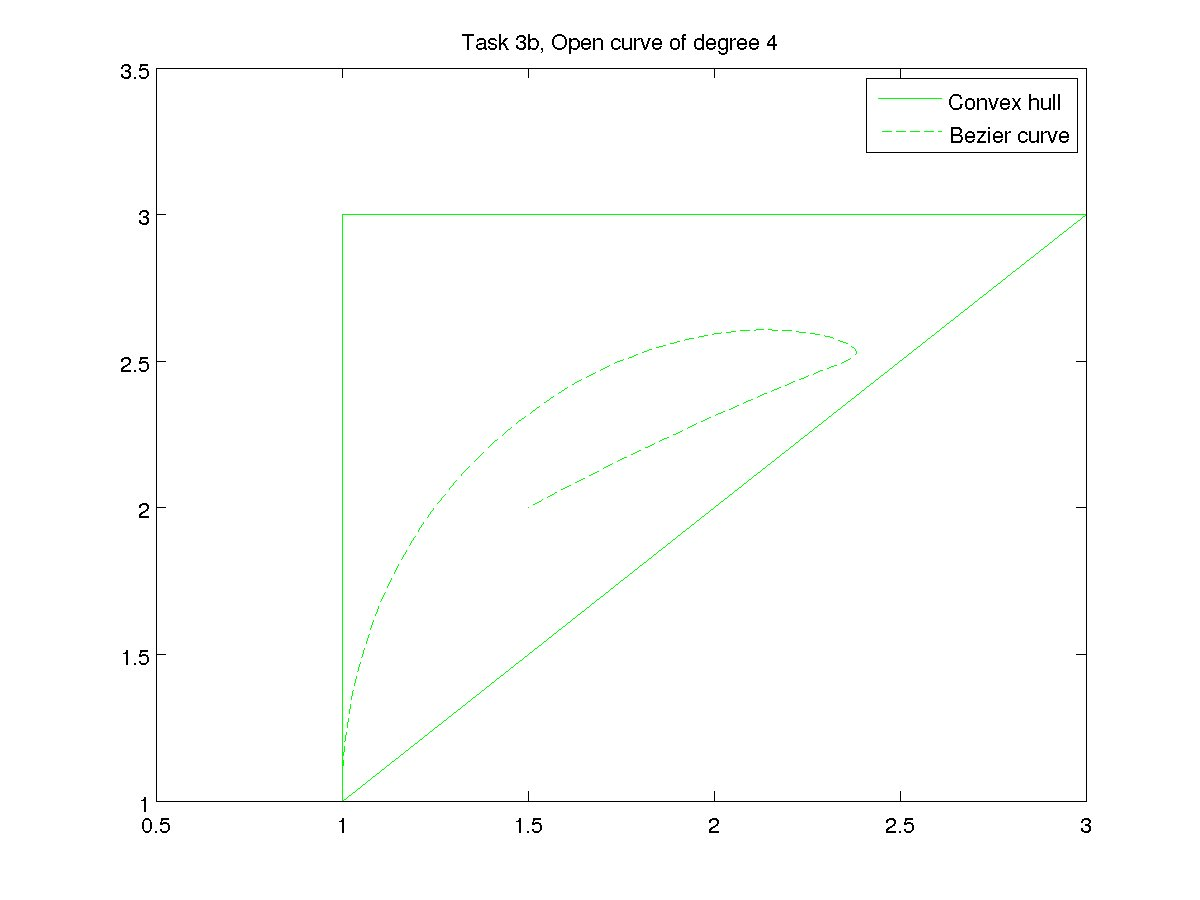
\includegraphics[scale=0.5]{task3b.jpg}
\end{center}
\end{figure}

\subsection{Task 3c}
 \label{task3c}
 \begin{figure}[H]
 \begin{center}
 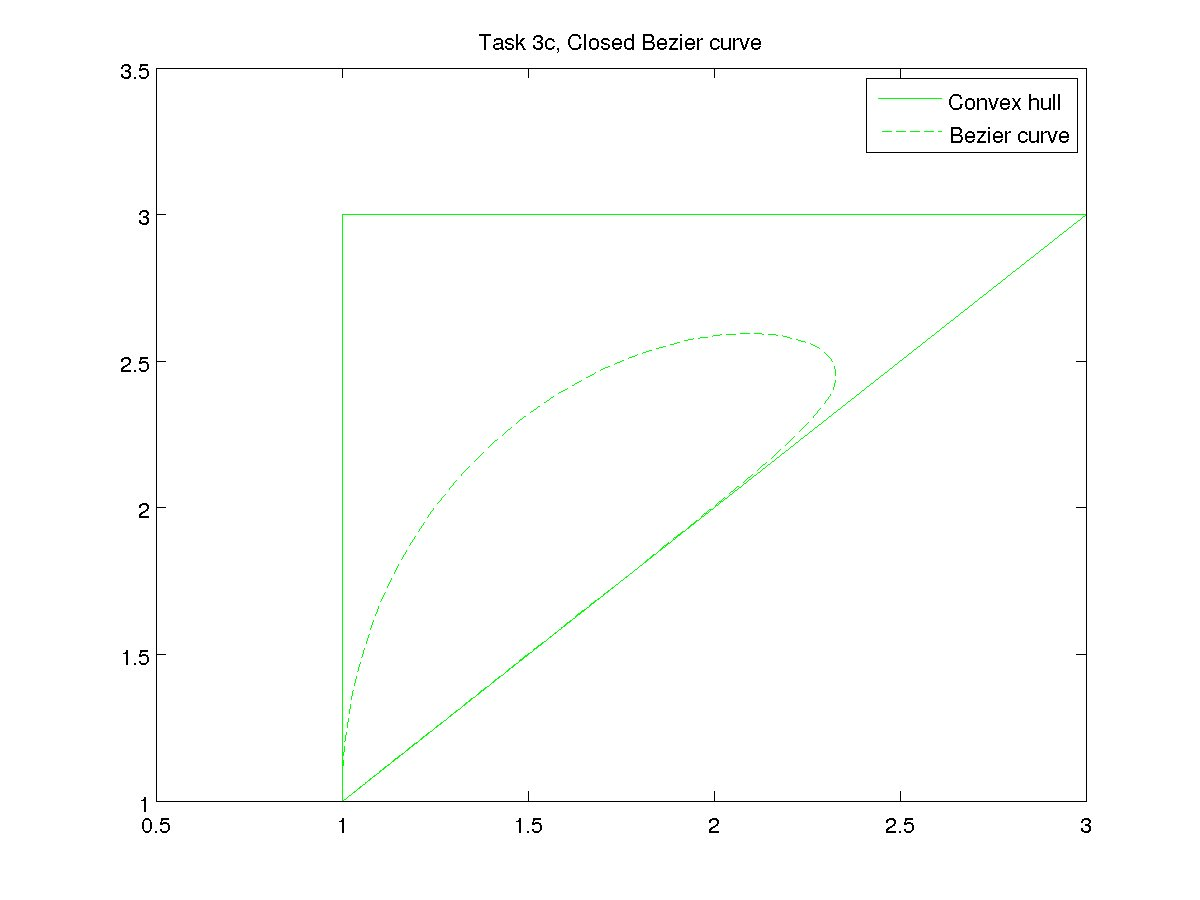
\includegraphics[scale=0.5]{task3c.jpg}
 \end{center}
 \end{figure}
\newpage

 \subsection{Task 3d}
\label{task3d}
\begin{figure}[H]
\begin{center}
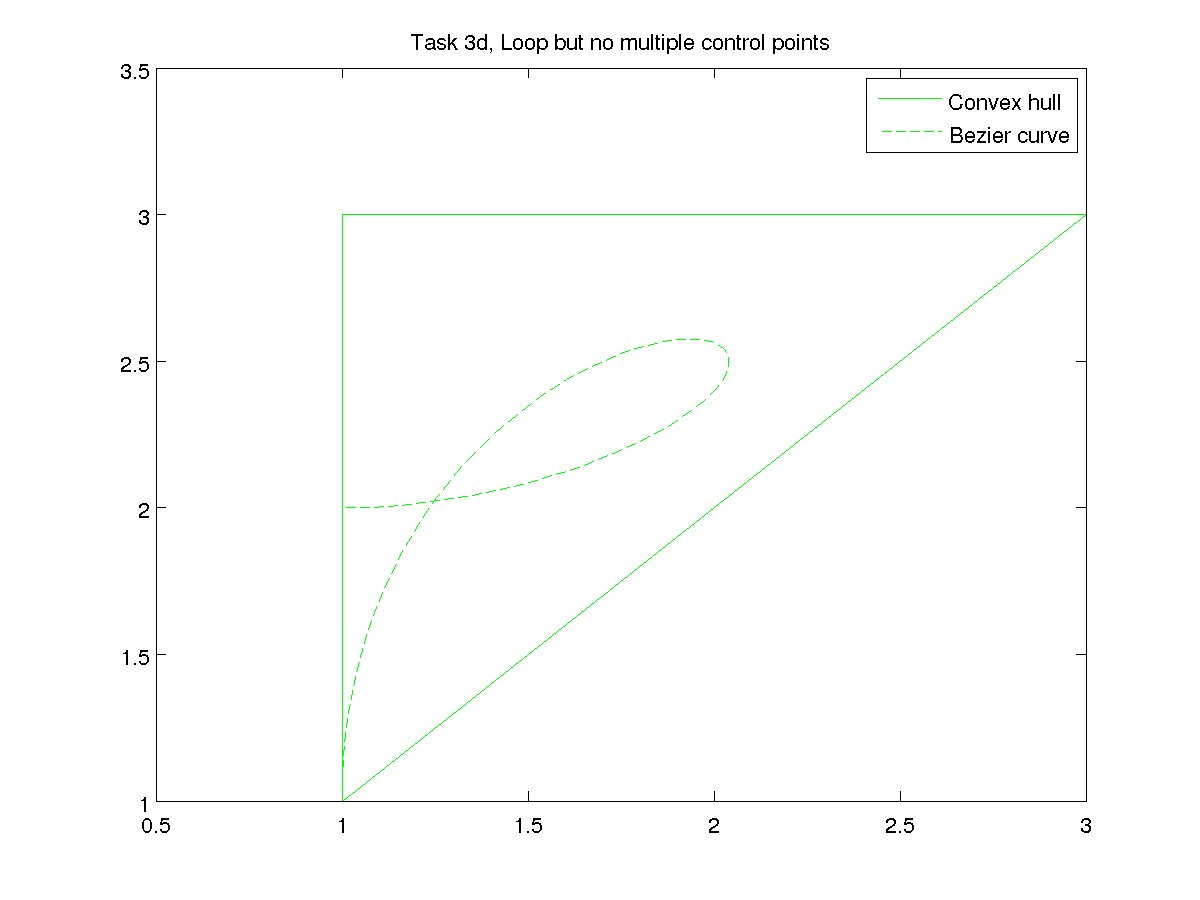
\includegraphics[scale=0.5]{task3d.jpg}
\end{center}
\end{figure}

\subsection{Task 3e}
 \label{task3e}
 \begin{figure}[H]
 \begin{center}
 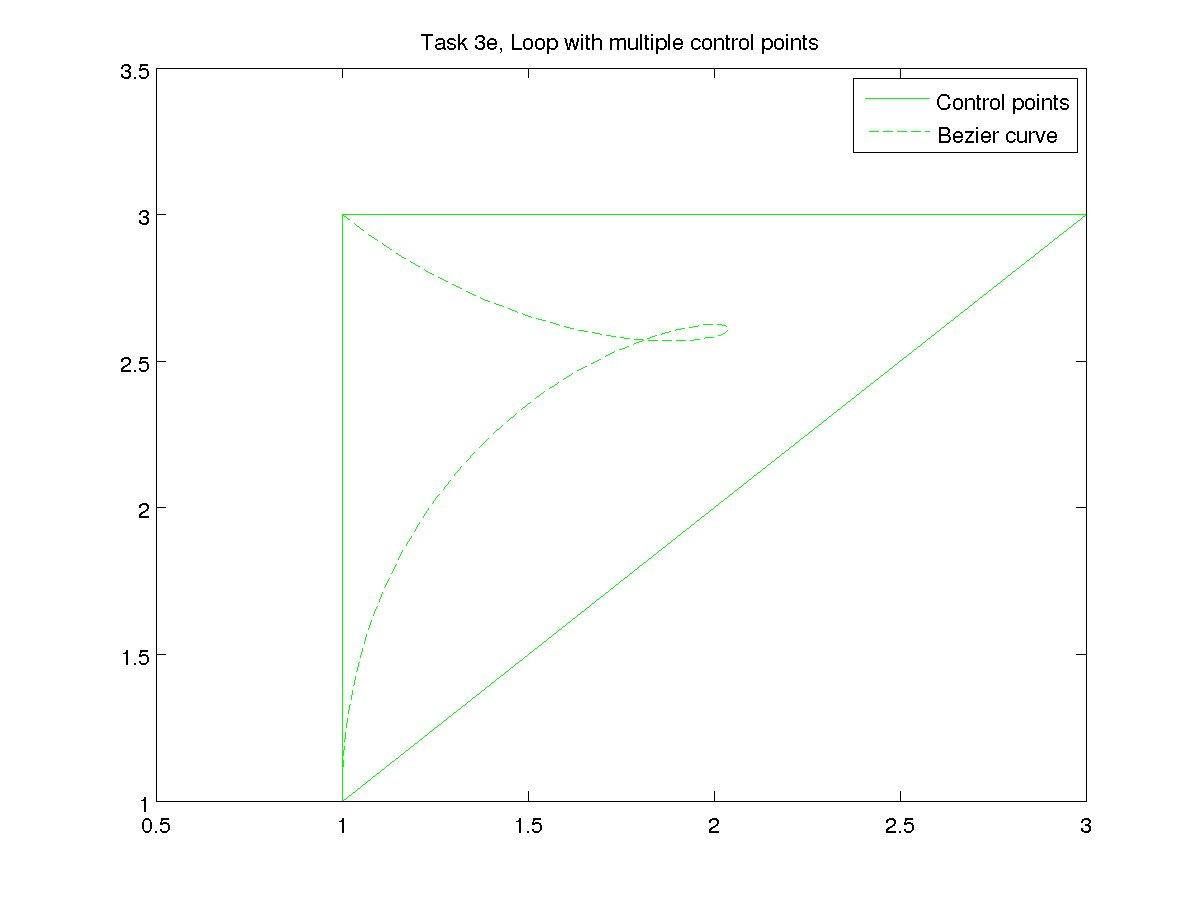
\includegraphics[scale=0.5]{task3e.jpg}
 \end{center}
 \end{figure}
\newpage

 \subsection{Task 4a}
\label{task4a}
\begin{figure}[H]
\begin{center}
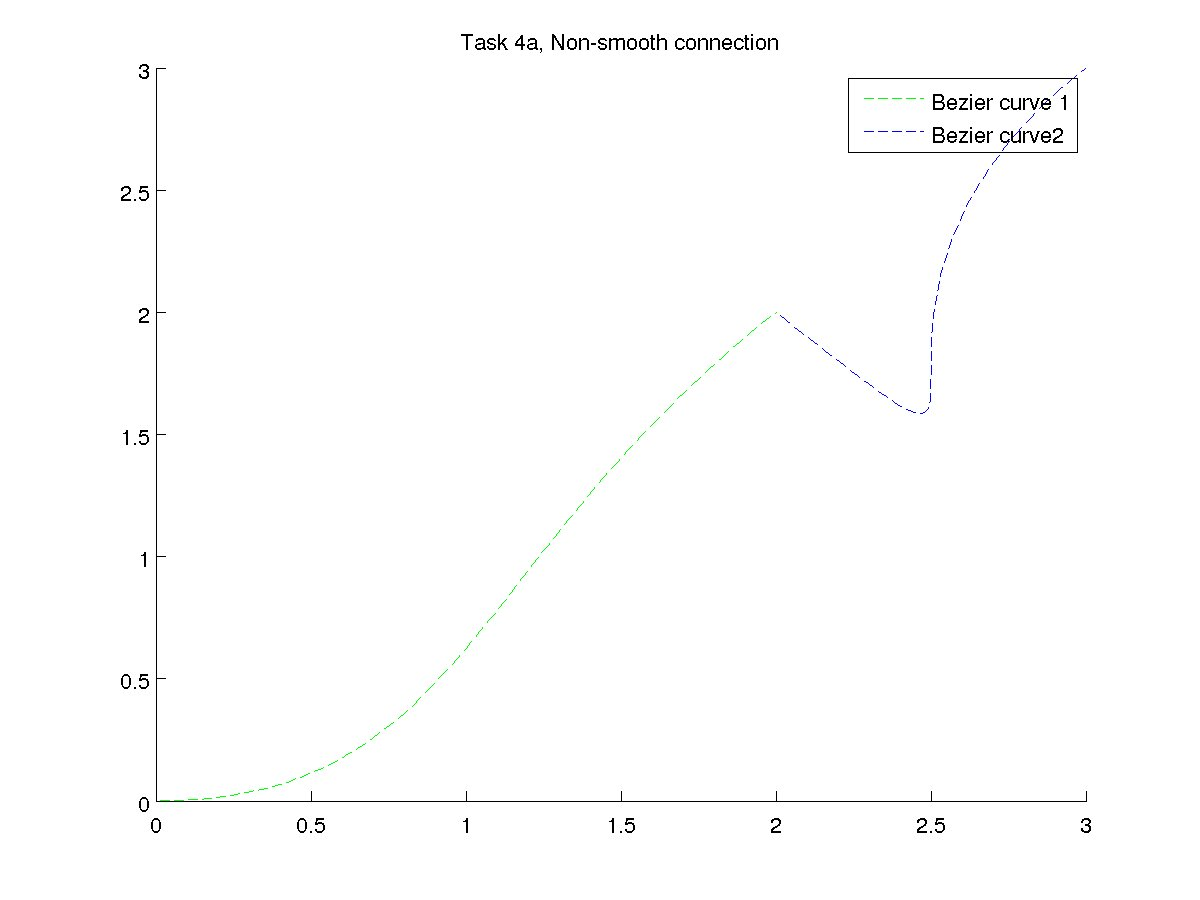
\includegraphics[scale=0.5]{task4a.jpg}
\end{center}
\end{figure}

\subsection{Task 4b}
 \label{task4b}
 \begin{figure}[H]
 \begin{center}
 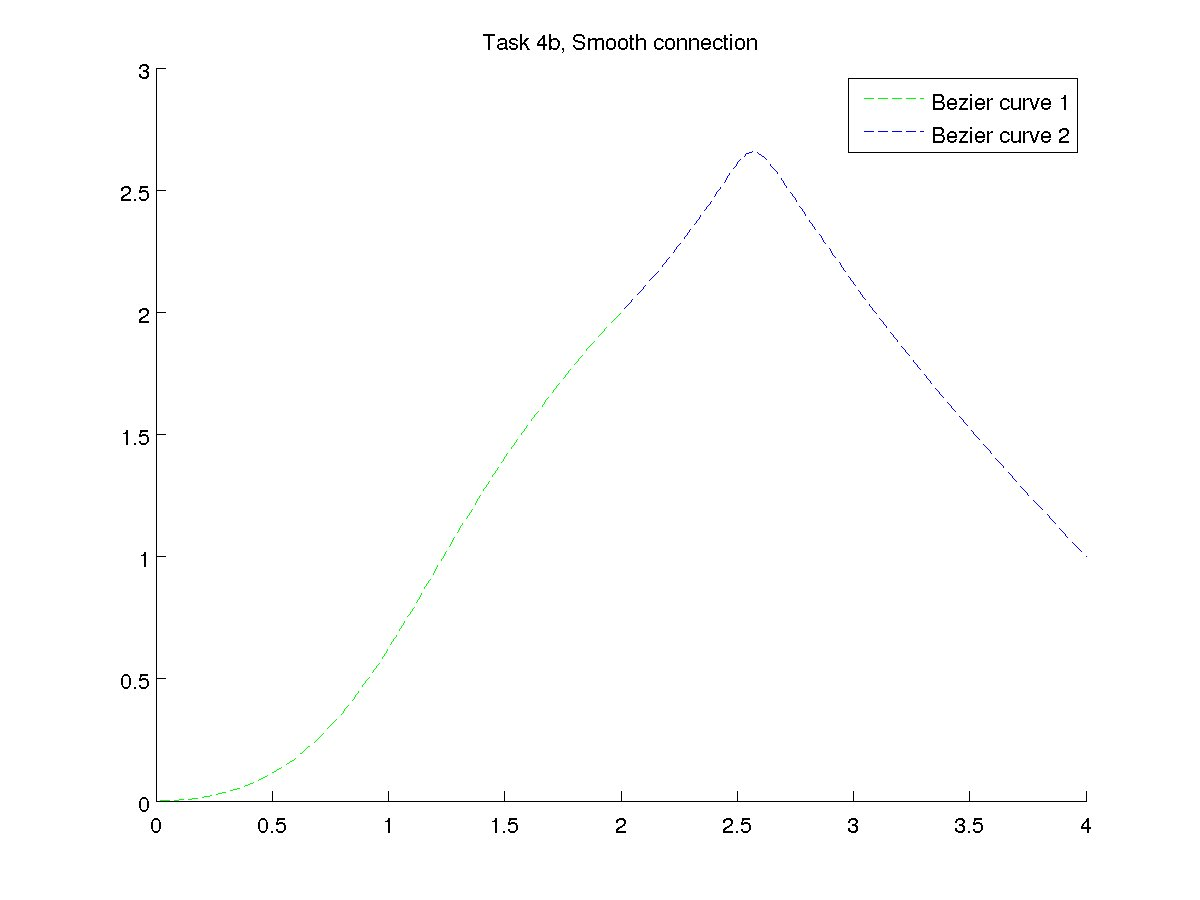
\includegraphics[scale=0.5]{task4b.jpg}
 \end{center}
 \end{figure}
\newpage

 \subsection{Task 5}
\label{task5}
\begin{figure}[H]
\begin{center}
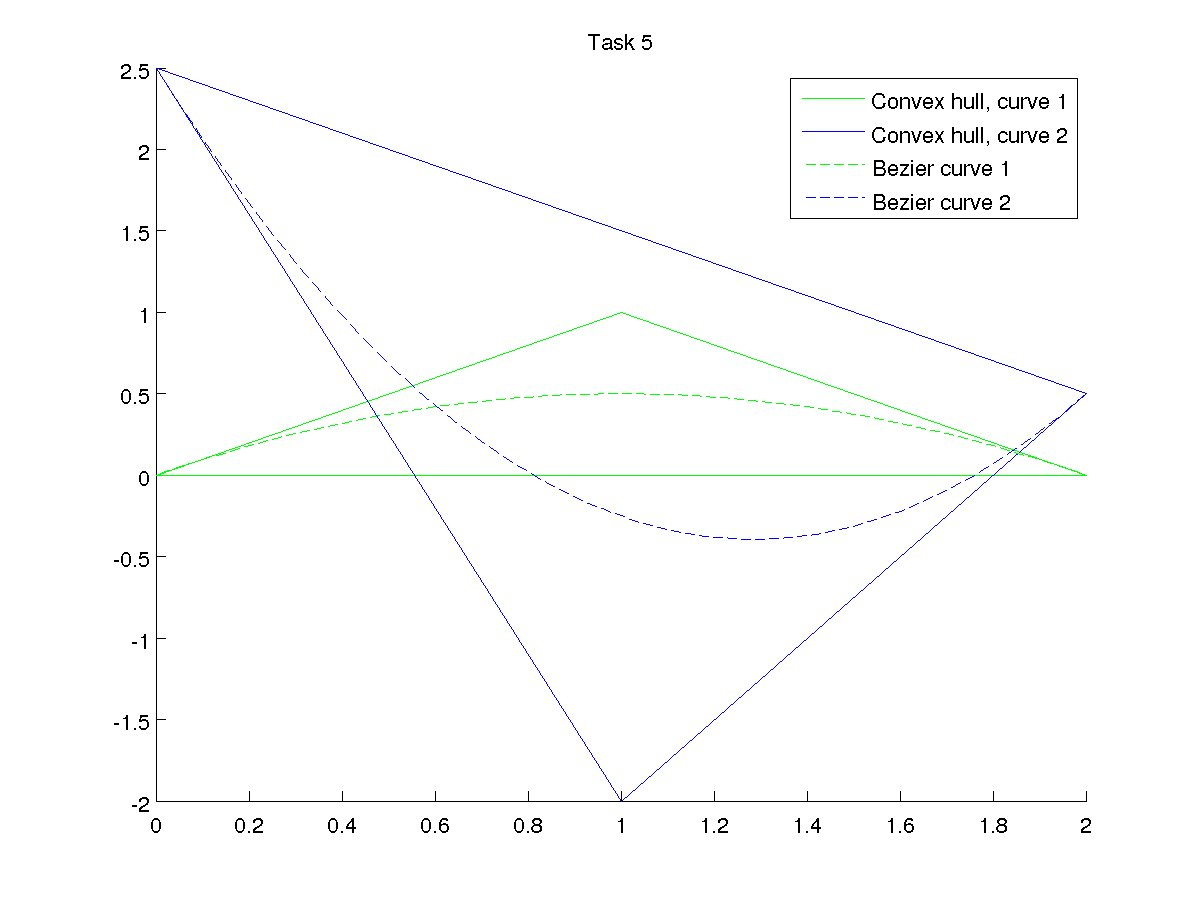
\includegraphics[scale=0.5]{task5.jpg}
\end{center}
\end{figure}

\subsection{Task 6}
 \label{task6}
 \begin{figure}[H]
 \begin{center}
 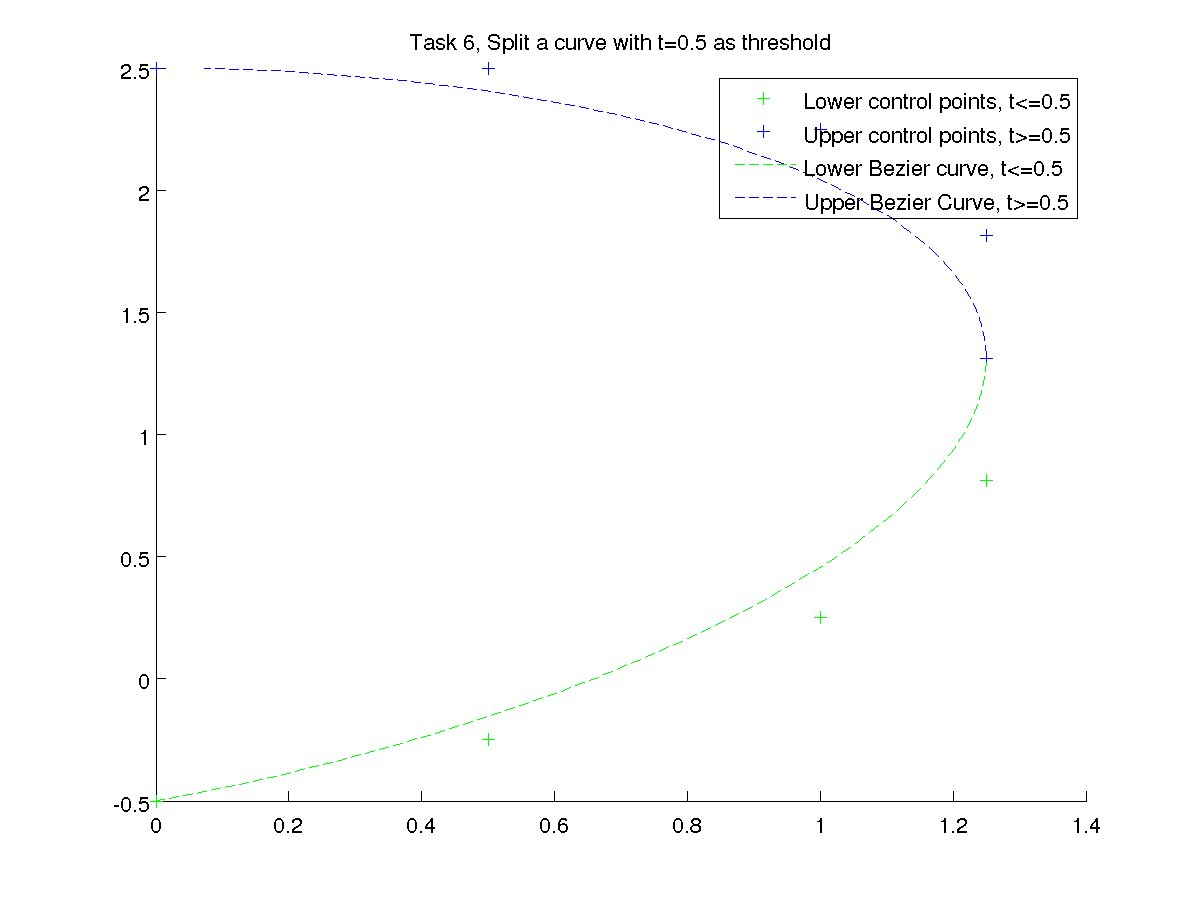
\includegraphics[scale=0.5]{task6.jpg}
 \end{center}
 \end{figure}
\newpage

 \subsection{Task 7}
\label{task7}
\begin{figure}[H]
\begin{center}
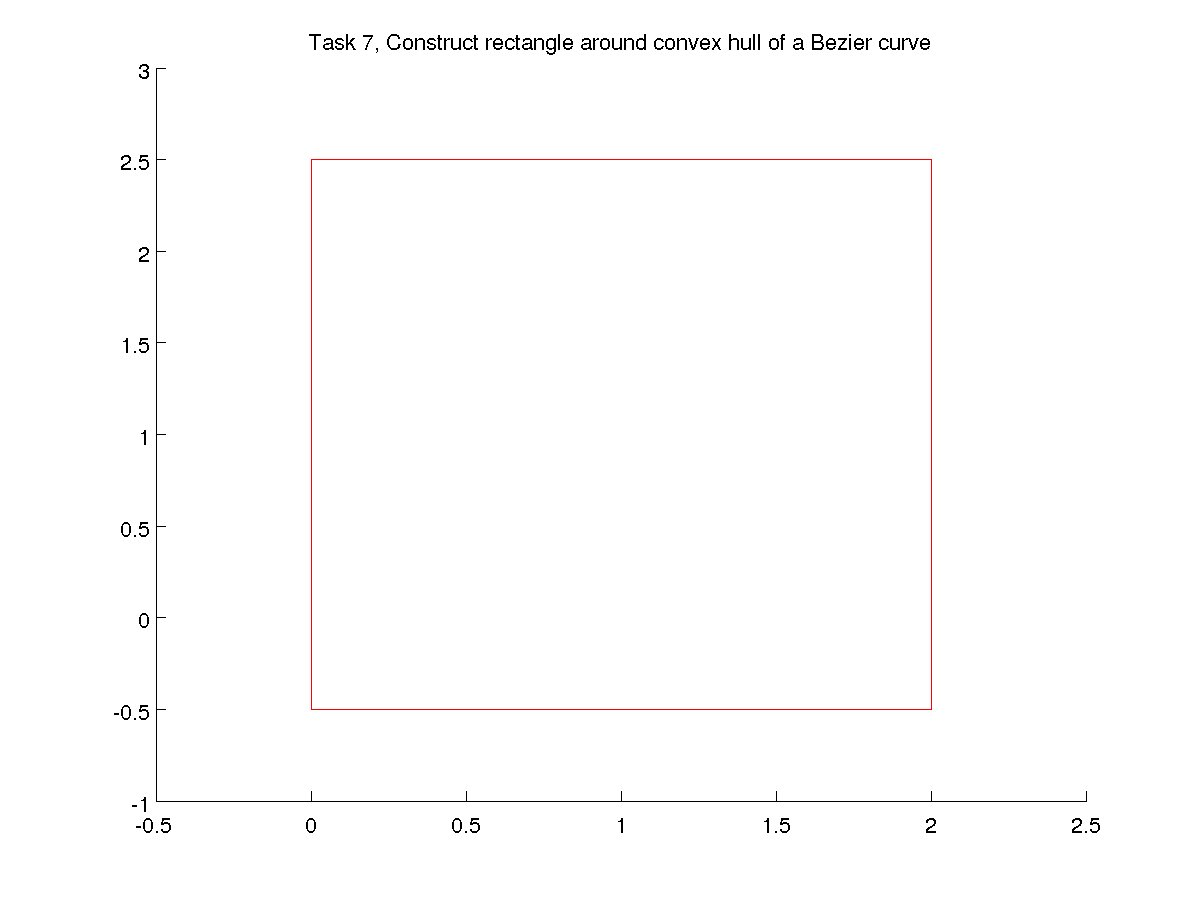
\includegraphics[scale=0.5]{task7.jpg}
\end{center}
\end{figure}

\subsection{Task 8}
 \label{task8}
 \begin{figure}[H]
 \begin{center}
 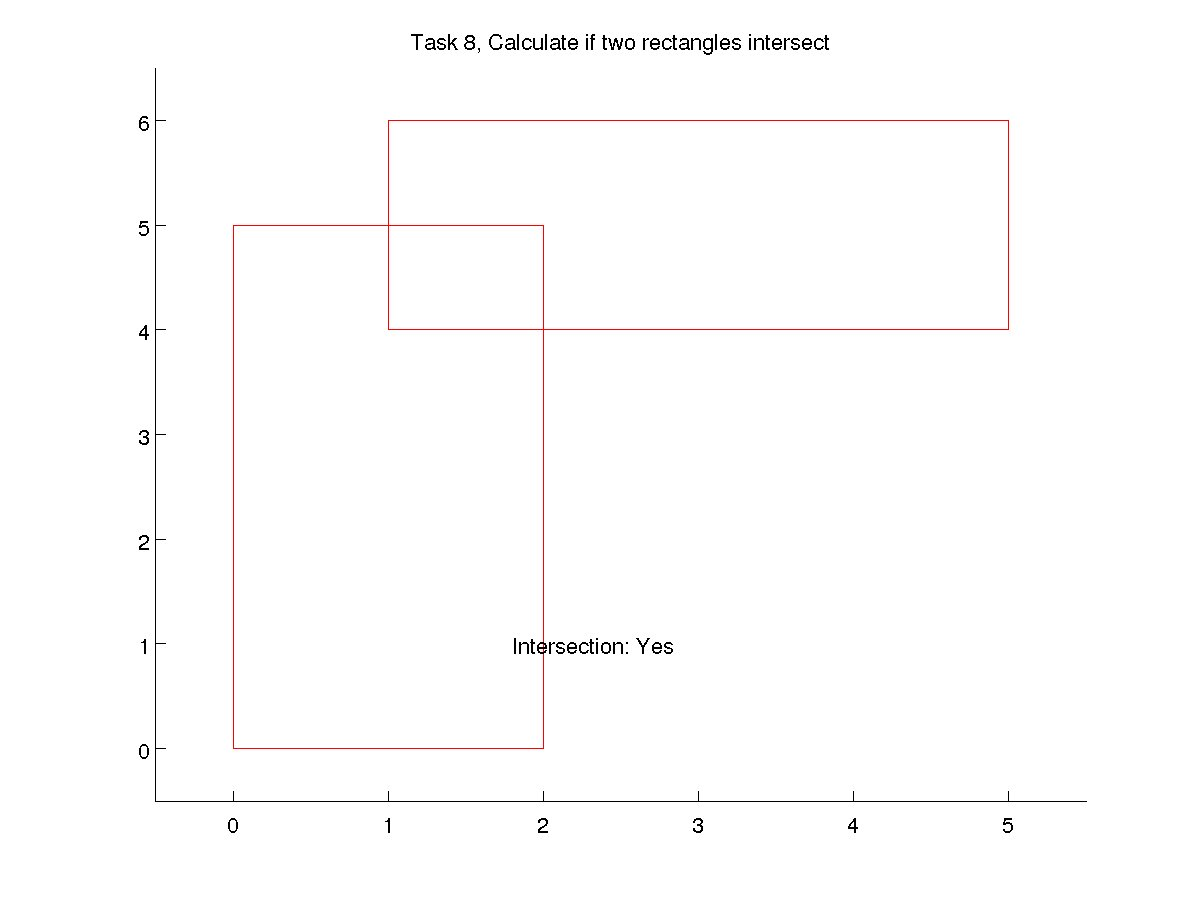
\includegraphics[scale=0.5]{task8.jpg}
 \end{center}
 \end{figure}
\newpage

 \subsection{Task 9a}
\label{task9a}
\begin{figure}[H]
\begin{center}
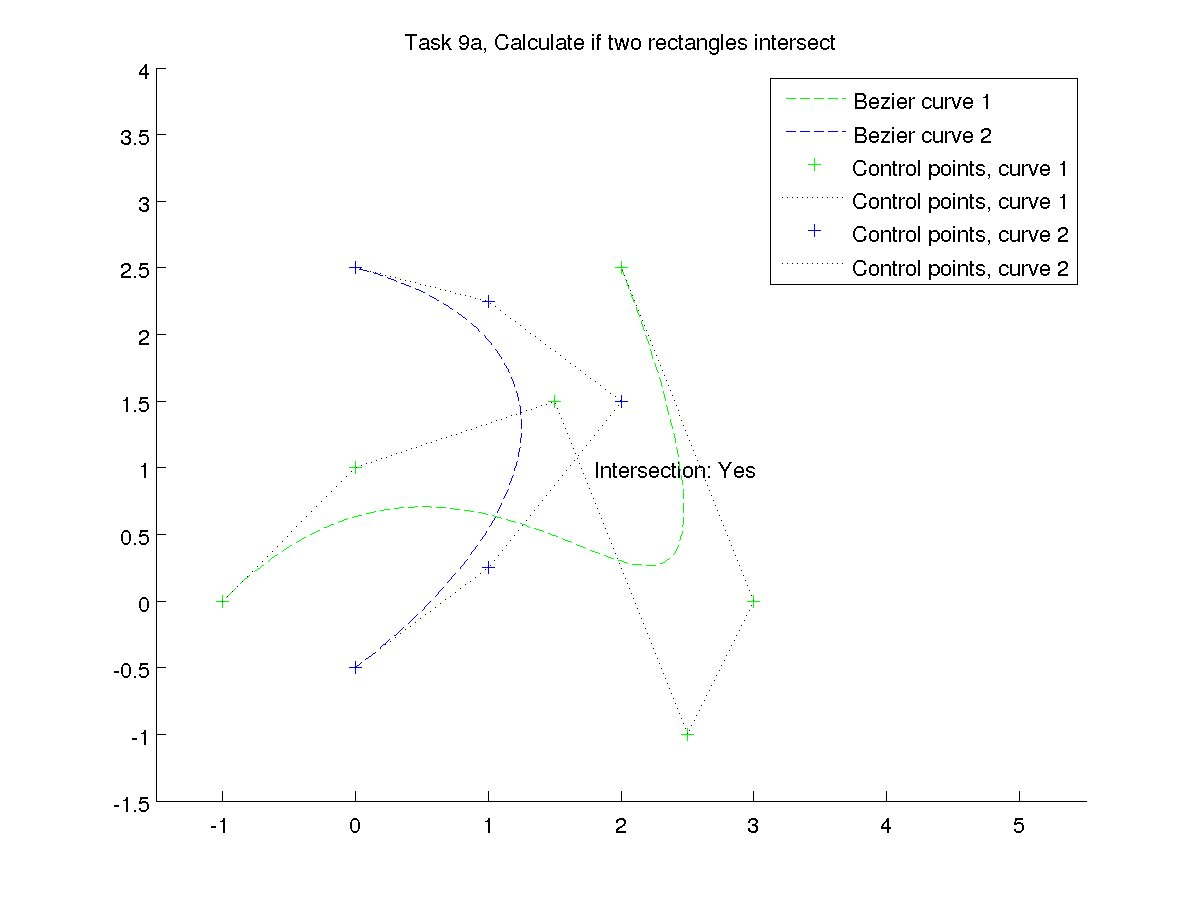
\includegraphics[scale=0.5]{task9a.jpg}
\end{center}
\end{figure}

\subsection{Task 9b}
 \label{task9b}
 \begin{figure}[H]
 \begin{center}
 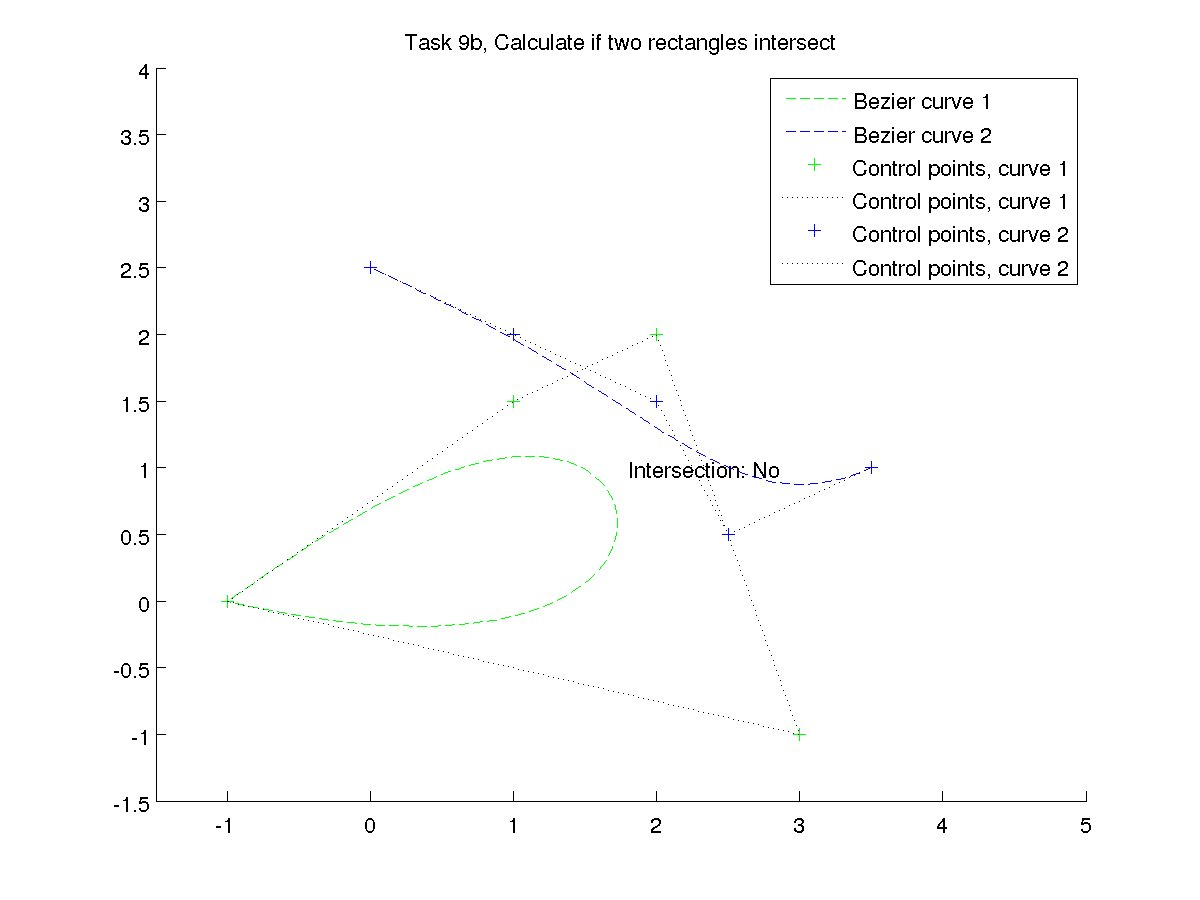
\includegraphics[scale=0.5]{task9b.jpg}
 \end{center}
 \end{figure}
\newpage

\subsection{Task 10a}
\label{task10a}
\begin{figure}[H]
\begin{center}
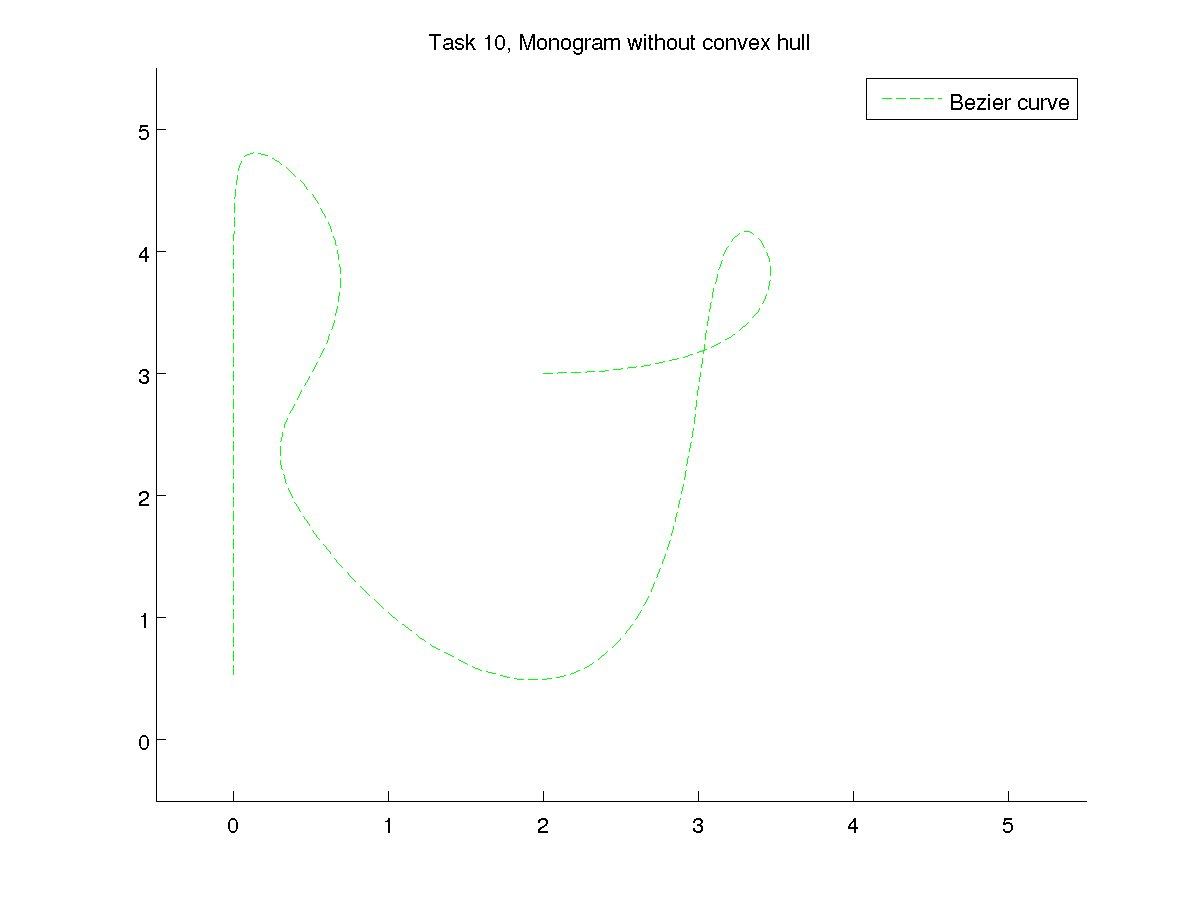
\includegraphics[scale=0.5]{task10a.jpg}
\end{center}
\end{figure}

\subsection{Task 10b}
 \label{task10b}
 \begin{figure}[H]
 \begin{center}
 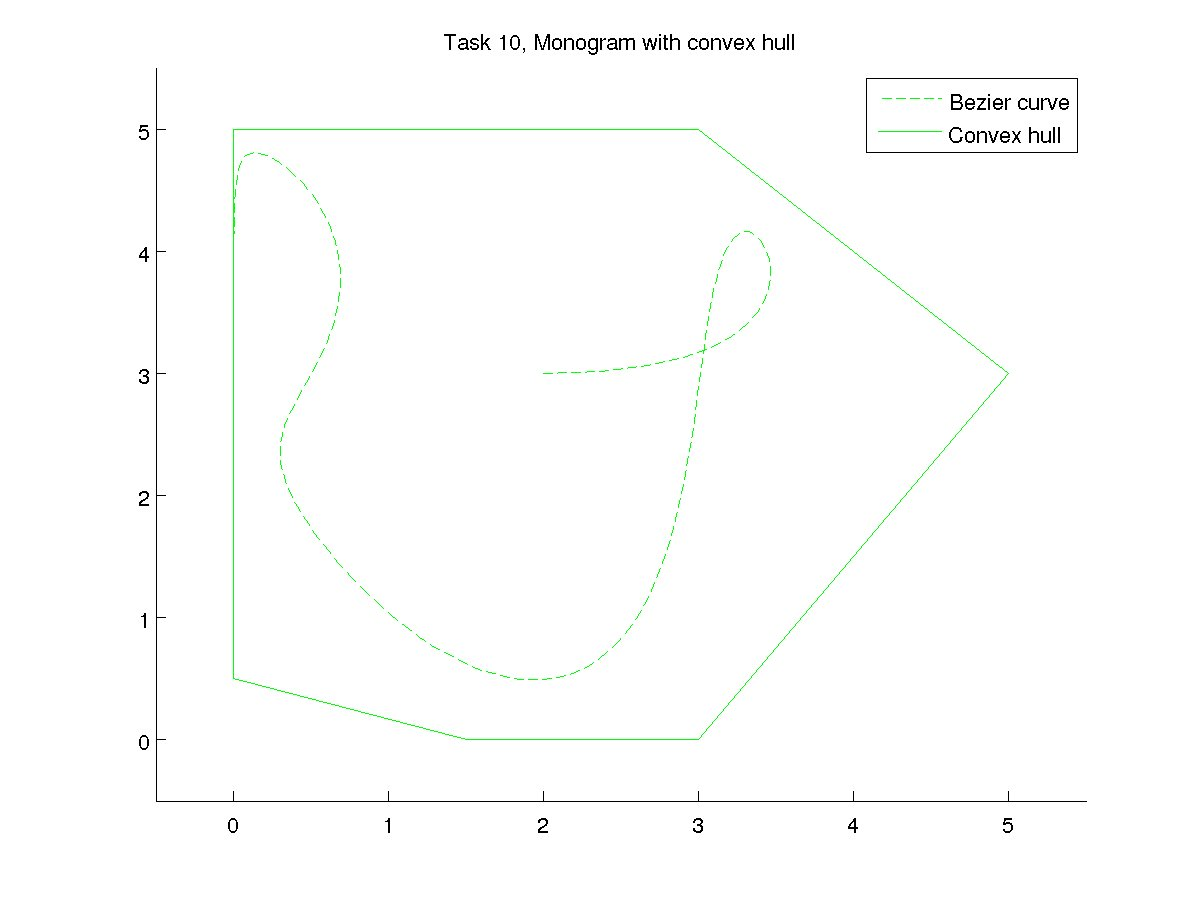
\includegraphics[scale=0.5]{task10b.jpg}
 \end{center}
 \end{figure}
 
\newpage
\section{Appendix: C}
\subsection{Program listing}
\label{programlisting}
\scriptsize
\verbatiminput{run.m}


\end{document}

